\section{\scshape kNN - dodatkowe}

\subsection{Złożono"sć}
\begin{frame}{Złożono"sć obliczeniowa}
\begin{itemize}
	\item Niski koszt fazy uczenia się.
	\item Wysoki koszt klasyfikacji.
	\item $O(dn)$
\end{itemize}
\end{frame}

\note{Niski koszt w fazie uczenia się w przeciwieństwie do fazy klasyfikacji. \\
Należy znaleźć $k$ najbliższych sąsiadów w"sród dużego zbioru $n$ wektorów. Do złożono"sć obliczeniowa ro"snie wraz ze wzrostem $d$ wymiarów.}

\begin{frame}{Wielowymiarowo"sć}
\begin{itemize}
	\item Dobra wydajno"sć dla niewielkiej liczby wymiarów.
	\item Przy wielu wymiarach wszystkie punkty są od siebie odległe.
	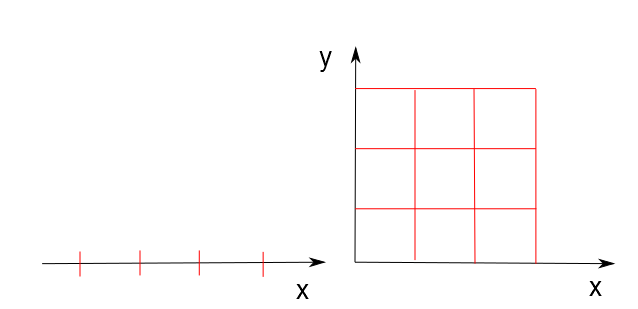
\includegraphics[keepaspectratio=true, scale=0.55]{dims_small}
\end{itemize}
\end{frame}

\note{Wraz ze wzrostem liczby wymiarów wydajno"sć kNN spada. \\
Nie tylko ze względu na zwiększenie liczby obliczeń potrzebnych do wyznaczenia dystansu. \\
Z każdym dodatkowym wymiarem, odległo"sc punktów od siebie wzrasta. Ilustrują to rysunki na slajdzie (dla $d = 1$ i $d = 2$). Utrudnia to klasyfikację.}


\subsection{Ważone kNN}
\begin{frame}{Ważone kNN}
\begin{itemize}
	\item Sąsiedzi położeni blisko mają większą wagę
	\item \textbf{Każdy} sąsiad bierze udział w etykietowaniu.
	\item Decyduje ważona większo"sć.
\end{itemize}
\end{frame}

\note{Brany jest pod uwagę dystans do każdego elementu zbioru uczącego. \\
Występuje zróżnicowanie wag dla otrzymanych odległo"sci (mniejsza odległo"sć - większa waga). \\
Decyzje o klasyfikacji podejmuje się, wybierając etykietę, która charakteryzuje się ważoną większo"scią. }

\subsection{Zastosowanie}
\begin{frame}{Zastosowanie}
\begin{itemize}
	\item Sytuacje trudne do modelowania w klasyczny sposób.
	\item Zależno"sć między zmiennymi jest nietypowa.
	\item Metody klasyczne są bardziej użyteczne w przypadku niezłożono"sci relacji.
\end{itemize}
\end{frame}

\note{Algorytm kNN sprawdza się przypadkach, gdy zależno"sć między zmiennymi jest złożona lub nietypowa.\\
W przeciwnym wypadku lepiej zastosować metody klasyczne.}